\begin{frame}[fragile]
    \frametitle{High-level interface to SCF}
    \inputminted[frame=single,fontfamily=tt,fontsize=\footnotesize]{python}{examples/hscf1.py}

    \begin{block}{Limitations}
        \begin{itemize}
            \item Rectangular container (i.e. an instance of the pirs.solids.Box() class)
            \item Rods inserted into grid element centers, no empty grid elements.
            \item Container and rods (and all internal structure) have the same height.
        \end{itemize}
    \end{block}
\end{frame}

\begin{frame}[fragile]
    \frametitle{SCF input file: channels}
    \inputminted[frame=single,fontfamily=tt,fontsize=\tiny,firstline=92,lastline=117]{rst}{examples/s1_0/input.txt}
\end{frame}

\begin{frame}[fragile]
    \frametitle{SCF input file: rods}
    \inputminted[frame=single,fontfamily=tt,fontsize=\tiny,firstline=152,lastline=166]{rst}{examples/s1_0/input.txt}
\end{frame}

\begin{frame}[fragile]
    \frametitle{SCF input file: power axial profile}
    \inputminted[frame=single,fontfamily=tt,fontsize=\tiny,firstline=343,lastline=362]{rst}{examples/s1_0/input.txt}
\end{frame}

\begin{frame}[fragile]
    \frametitle{SCF-specific parameters}
    \inputminted[frame=single,fontfamily=tt,fontsize=\tiny]{python}{examples/hscf2.py}
\end{frame}


\begin{frame}[fragile]
    \frametitle{SCF-specific parameters: rod material specifications}
    \inputminted[frame=single,fontfamily=tt,fontsize=\tiny]{python}{examples/hscf3.py}
\end{frame}

\begin{frame}[fragile]
    \frametitle{SCF-specific parameters: SCF results}
    \begin{columns}
        \column{0.5\textwidth}
        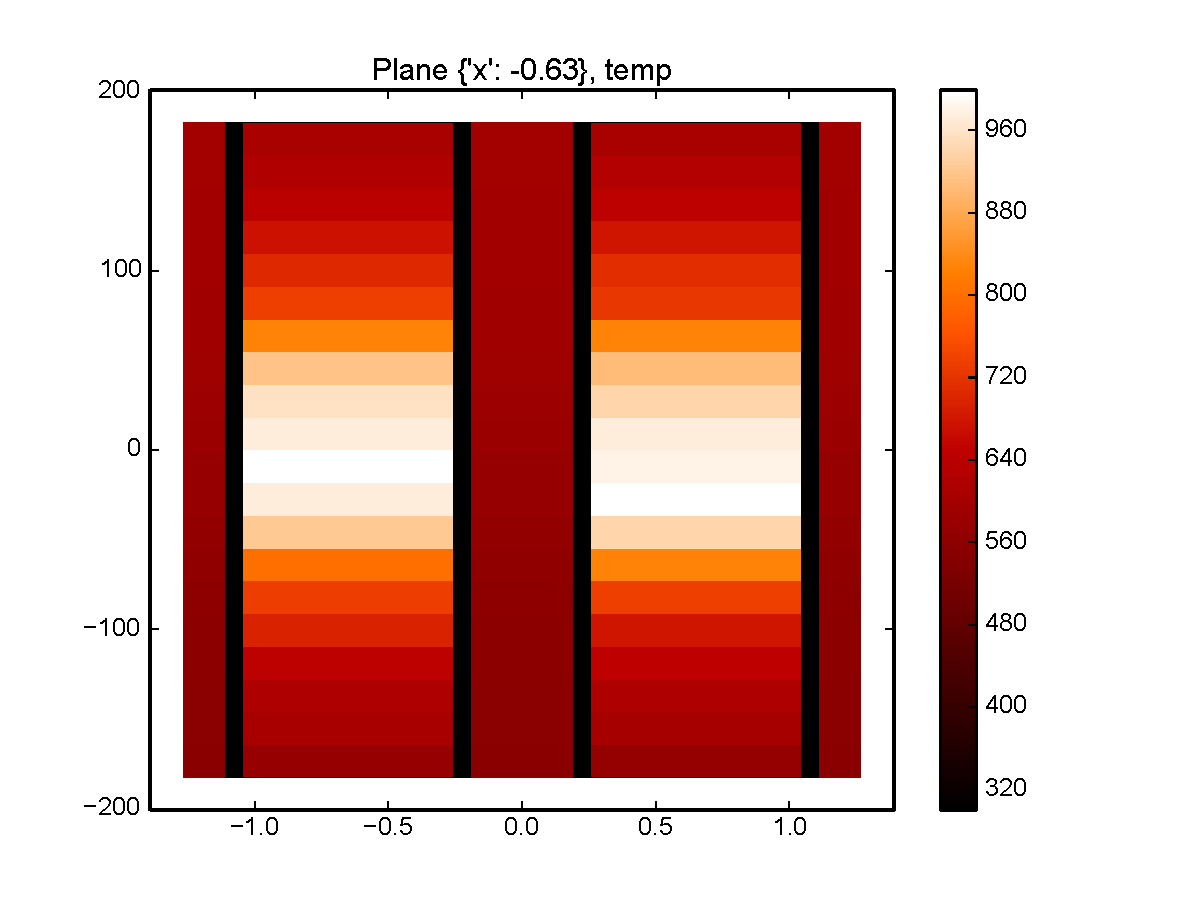
\includegraphics[width=\textwidth]{examples/hscf3_tx1.pdf}
        \column{0.5\textwidth}
        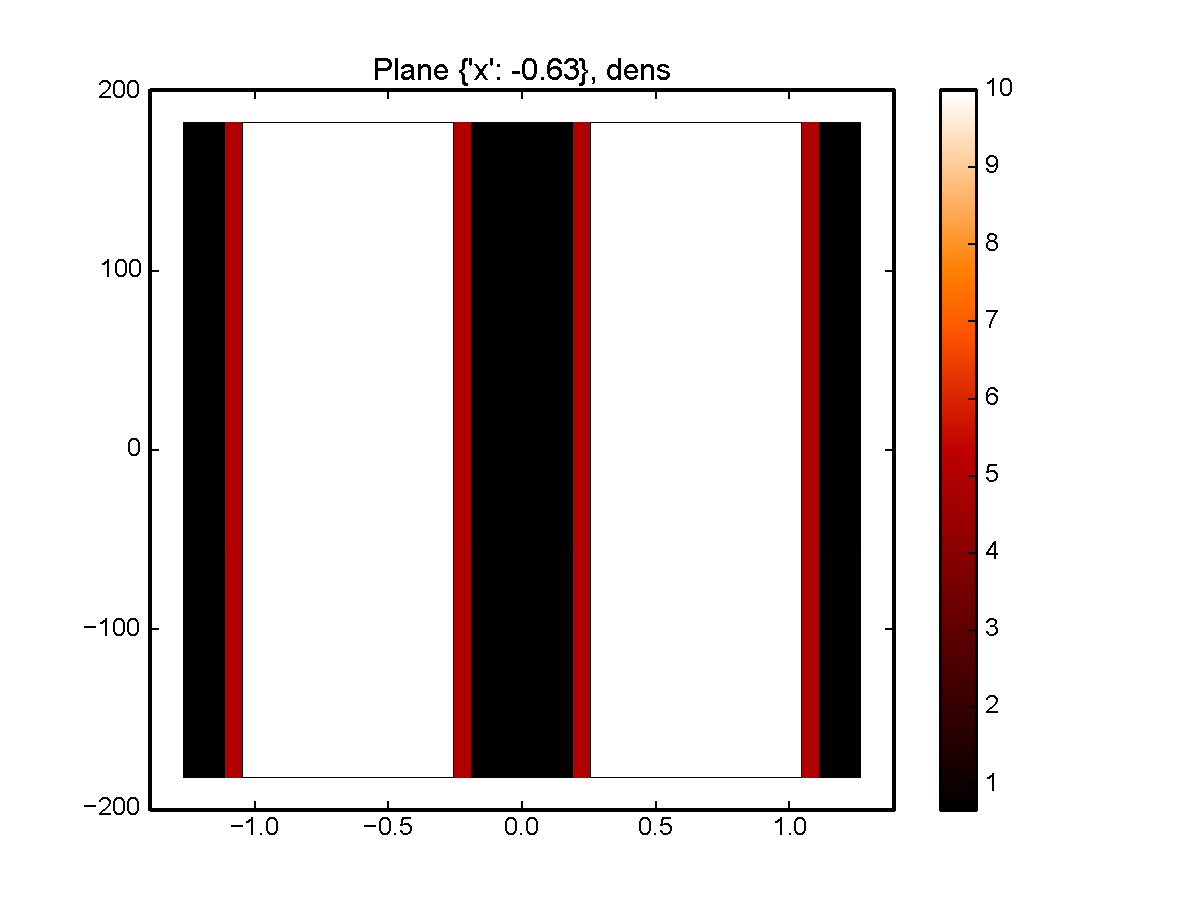
\includegraphics[width=\textwidth]{examples/hscf3_dx1.pdf}
    \end{columns}
\end{frame}


\begin{frame}[fragile]
    \frametitle{Data exchange between interfaces}
    \inputminted[frame=single,fontfamily=tt,fontsize=\tiny,lastline=27]{python}{examples/coupling.py}
\end{frame}

